\section{Программная реализация и тестирование}

Для визуализации работы алгоритма рассмотрим общую схему обмена ключами, представленную на рисунке~\ref{fig:keys_exchange}.

\begin{figure}[H]
\centering
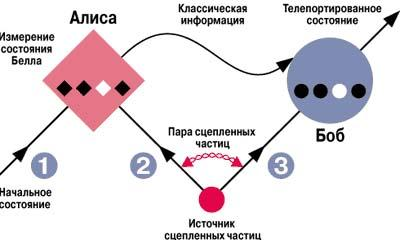
\includegraphics[scale=0.8]{img/keys.png}
\caption{Схема обмена асимметричными ключами}
\label{fig:keys_exchange}
\end{figure}

В процессе передачи информации данные преобразуются согласно схеме шифрования, проиллюстрированной на рисунке~\ref{fig:encryption_schema}.

\begin{figure}[H]
\centering
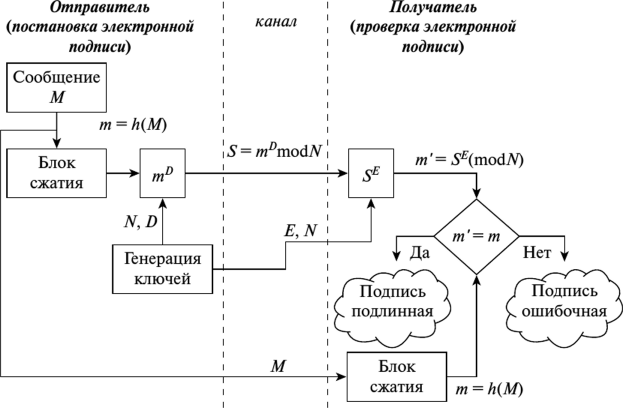
\includegraphics[scale=0.8]{img/schema.png}
\caption{Схема процесса шифрования и расшифрования RSA}
\label{fig:encryption_schema}
\end{figure}

Программная реализация алгоритма генерации ключей, шифрования и расшифрования на языке программирования Python~\cite{python_docs} вынесена в отдельный файл. Исходный код представлен ниже.

\inputminted{python}{src/rsa.py}

Для проверки корректности работы реализованного алгоритма было проведено тестирование на наборе входных данных. Результаты тестирования для различных исходных сообщений \texttt{m} и параметров ключей приведены в таблице~\ref{tab:test_results}.

\begin{table}[H]
\centering
\caption{Результаты тестирования алгоритма RSA}
\label{tab:test_results}
\begin{tabular}{|c|c|c|c|c|}
\hline
$p$ & $q$ & Исходное сообщение $m$ & Шифротекст $c$ & Расшифрованное сообщение \\
\hline
61 & 53 & 65 & 2790 & 65 \\
17 & 19 & 88 & 192 & 88 \\
23 & 29 & 42 & 101 & 42 \\
\hline
\end{tabular}
\end{table}
